\documentclass[10pt, usenames, dvipsnames, table]{beamer}
\usetheme{Berkeley}
\usecolortheme{beetle}
\usepackage{graphicx}
\graphicspath{ {../} }
\usepackage{array}
\RequirePackage{fix-cm}
\usepackage{colortbl}
\usepackage{hyperref}
\usepackage{graphbox}
\usepackage{algorithm}
\usepackage{algpseudocode}

\title{Query Selection based on Latent Space Sampling}
\author{Benjamin Killeen}
\date{}

\DeclareMathOperator{\kl}{KL}

\begin{document}

\begin{frame}
  \titlepage
\end{frame}

\begin{frame}
  \frametitle{Outline}
  \tableofcontents
\end{frame}


\section{Motivation}
\label{sec:motivation}

\begin{frame}
  \frametitle{Motivation: Supervised Learning}
  \begin{columns}
    \column{0.5\textwidth}
    \begin{itemize}
    \item<1-> \textbf{Big data} facilitates supervised learning.
    \item<3-> Labels are necessary for \textbf{specialized} tasks.
    \end{itemize}
    \vspace{2em}
    \onslide<3->{    
      \begin{figure}
        \centering
        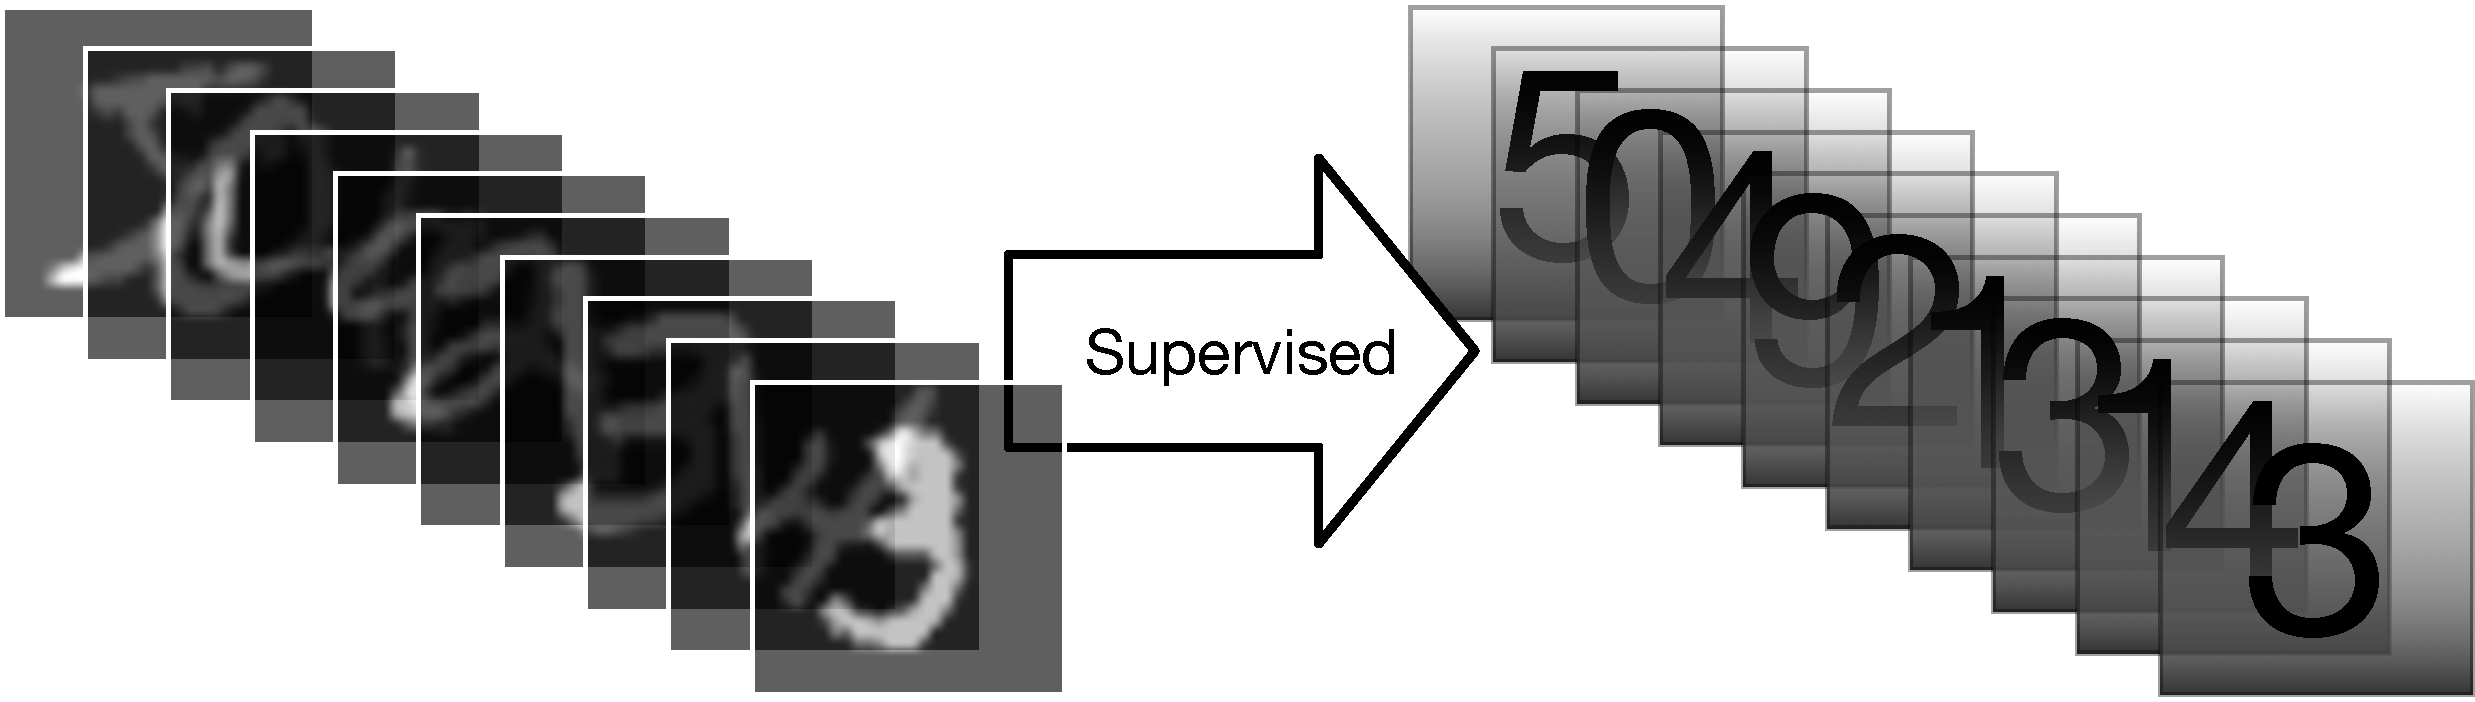
\includegraphics[width=\linewidth]{docs/supervised}
        \caption{MNIST classification \cite{lecun_gradient-based_1998}.}
        \label{fig:supervised}
      \end{figure}
    }
    \column{0.5\textwidth}
    \onslide<2->{
      \begin{figure}
        \centering
        \includegraphics[width=\linewidth]{docs/imagenet}
        \caption{ImageNet examples \cite{deng_imagenet:_nodate}.}
        \label{fig:imagenet}
      \end{figure}
    }
  \end{columns}
\end{frame}

\begin{frame}
  \frametitle{Unsupervised Learning}
  \begin{itemize}
  \item Understanding the underlying \textbf{structure} of data.
    \pause{}
  \item Avoids the high \textbf{cost} of labeling.
  \end{itemize}
  \pause{}
  \begin{figure}
    \centering
    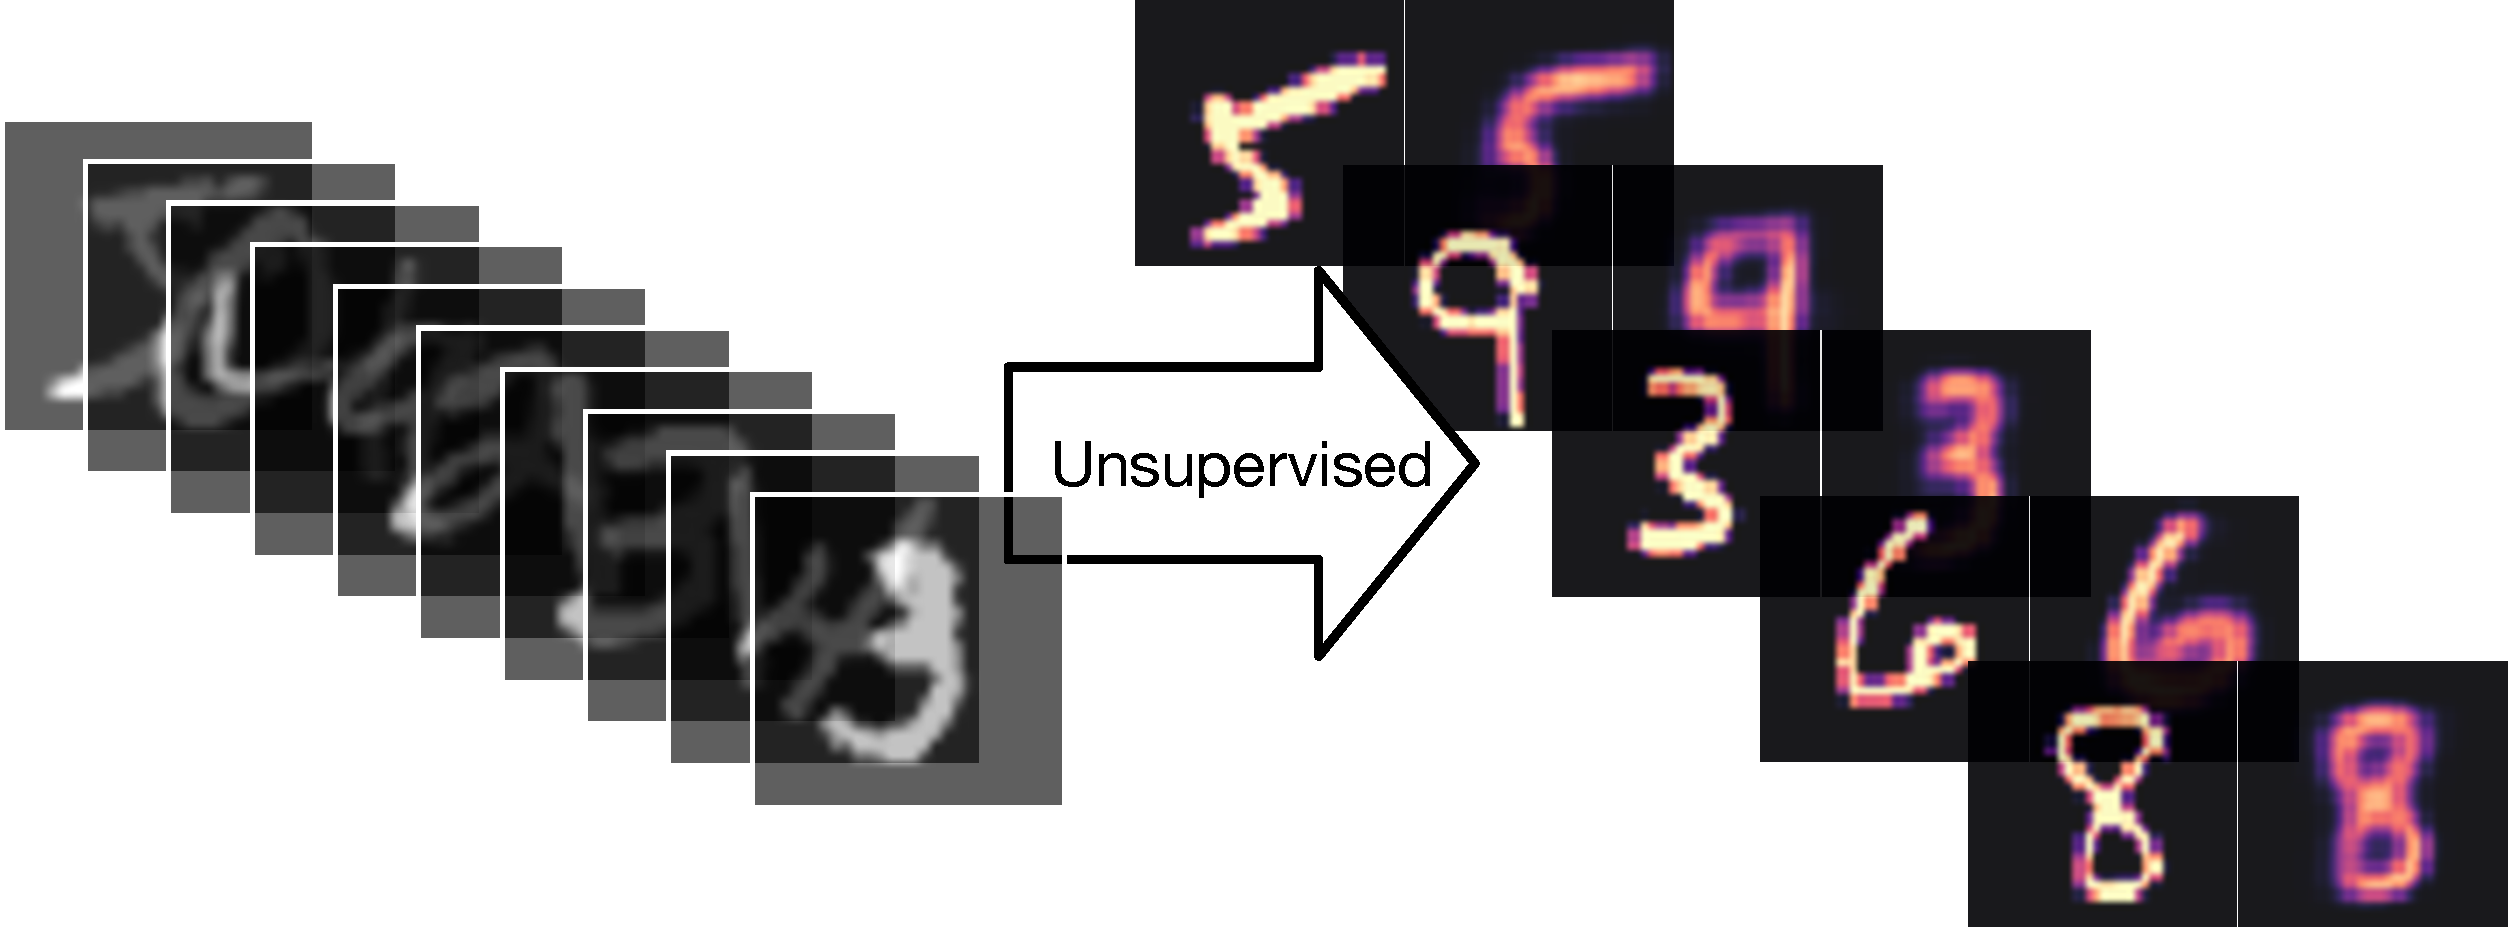
\includegraphics[align=c, width=0.4\linewidth]{docs/unsupervised}
    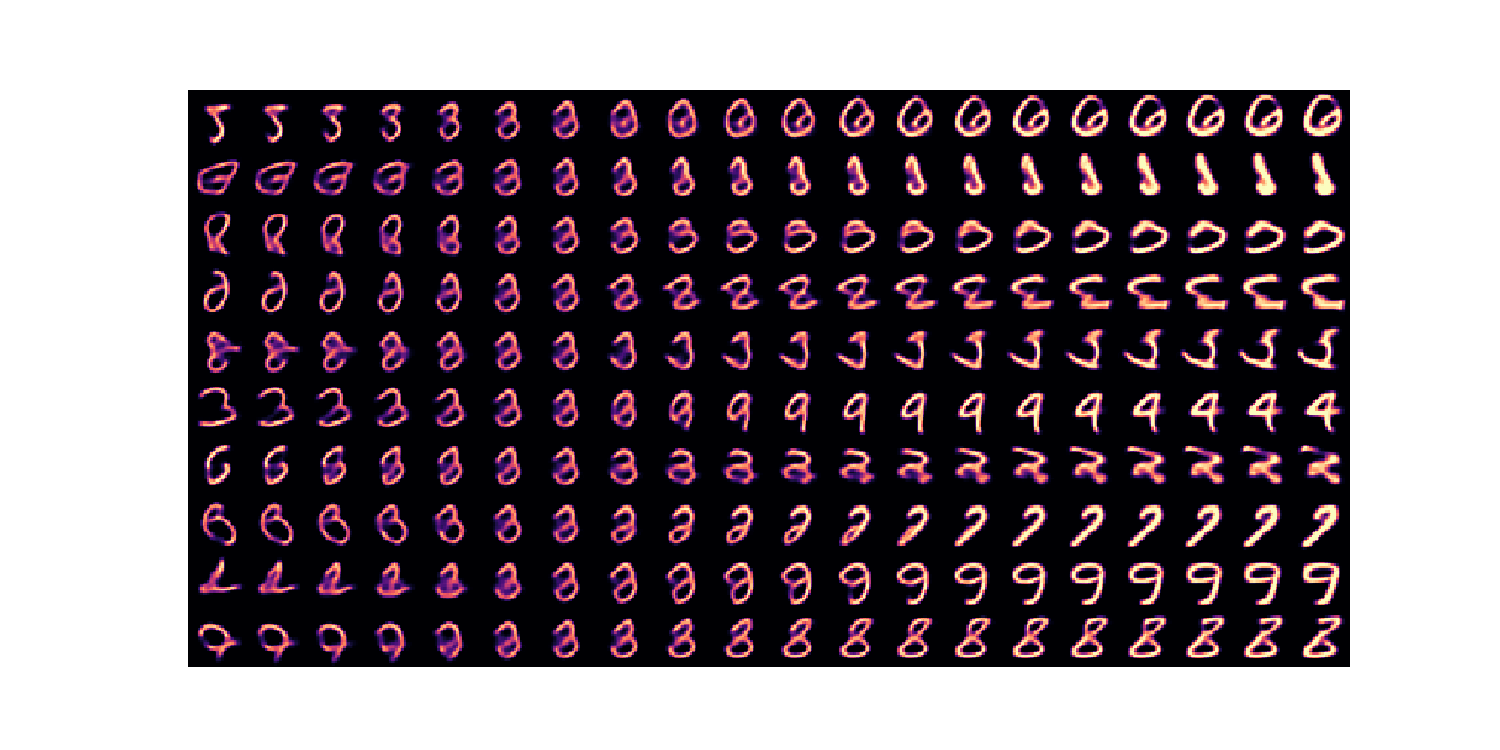
\includegraphics[align=c, width=0.55\linewidth]{docs/visualize_decoding}
    \caption{latent space learned by an auto-encoder.}
    \label{fig:unsupervised}
  \end{figure}
\end{frame}

\begin{frame}
  \frametitle{Semi-supervised Learning}
  \begin{figure}
    \centering
    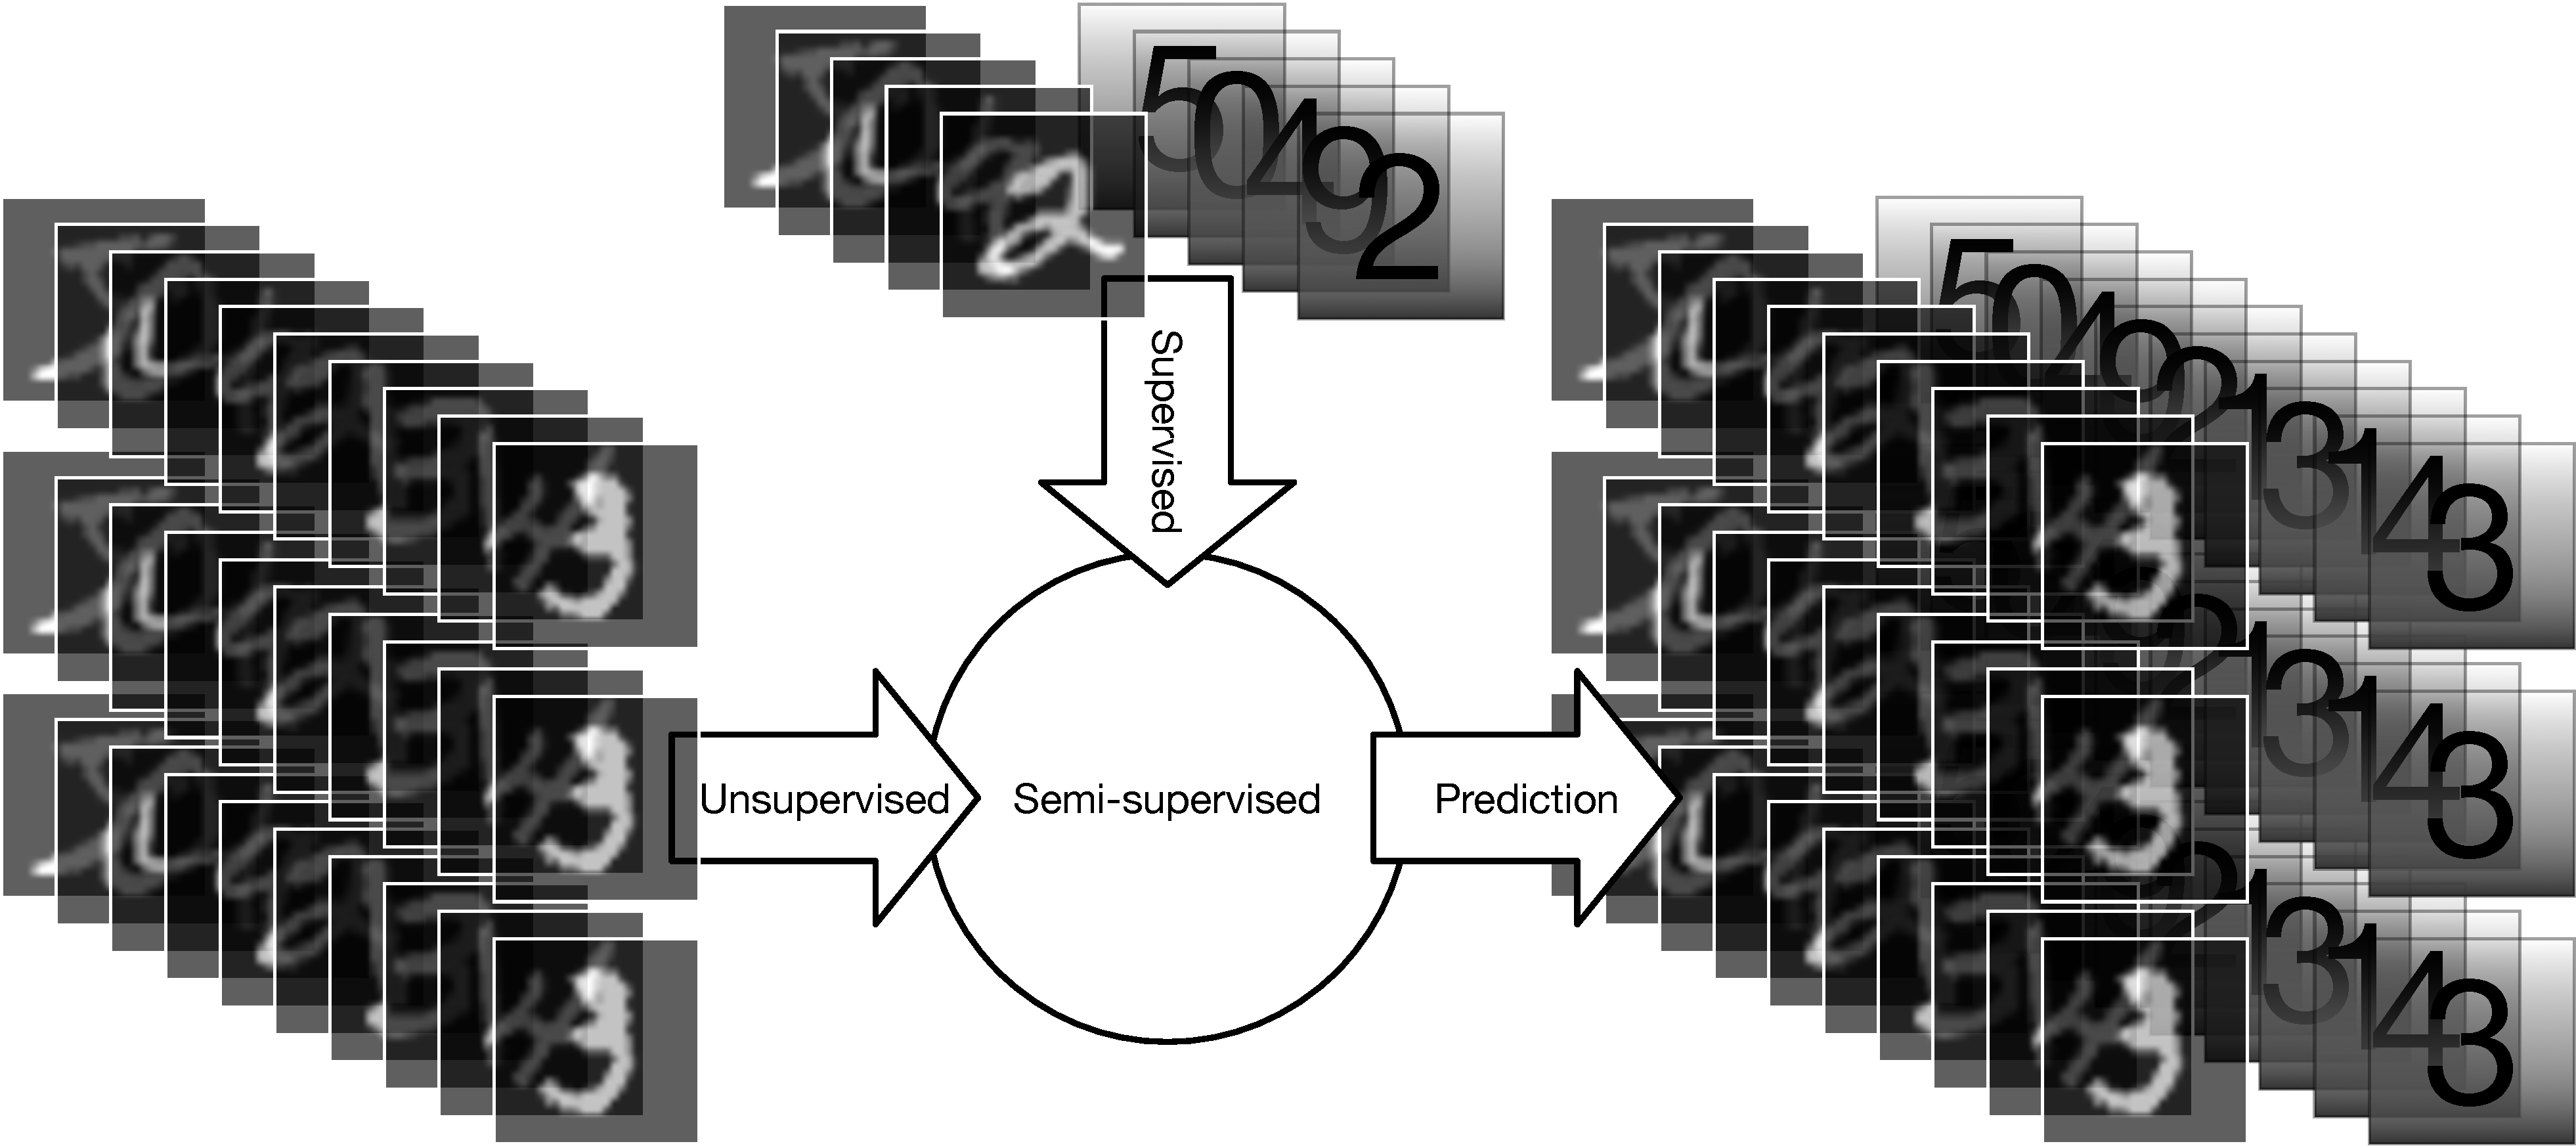
\includegraphics[width=\linewidth]{docs/semi_supervised}
    \caption{semi-supervised learning.}
    \label{fig:semi-supervised}
  \end{figure}
\end{frame}

\begin{frame}
  \frametitle{Starting from Scratch}
  \begin{figure}
    \centering
    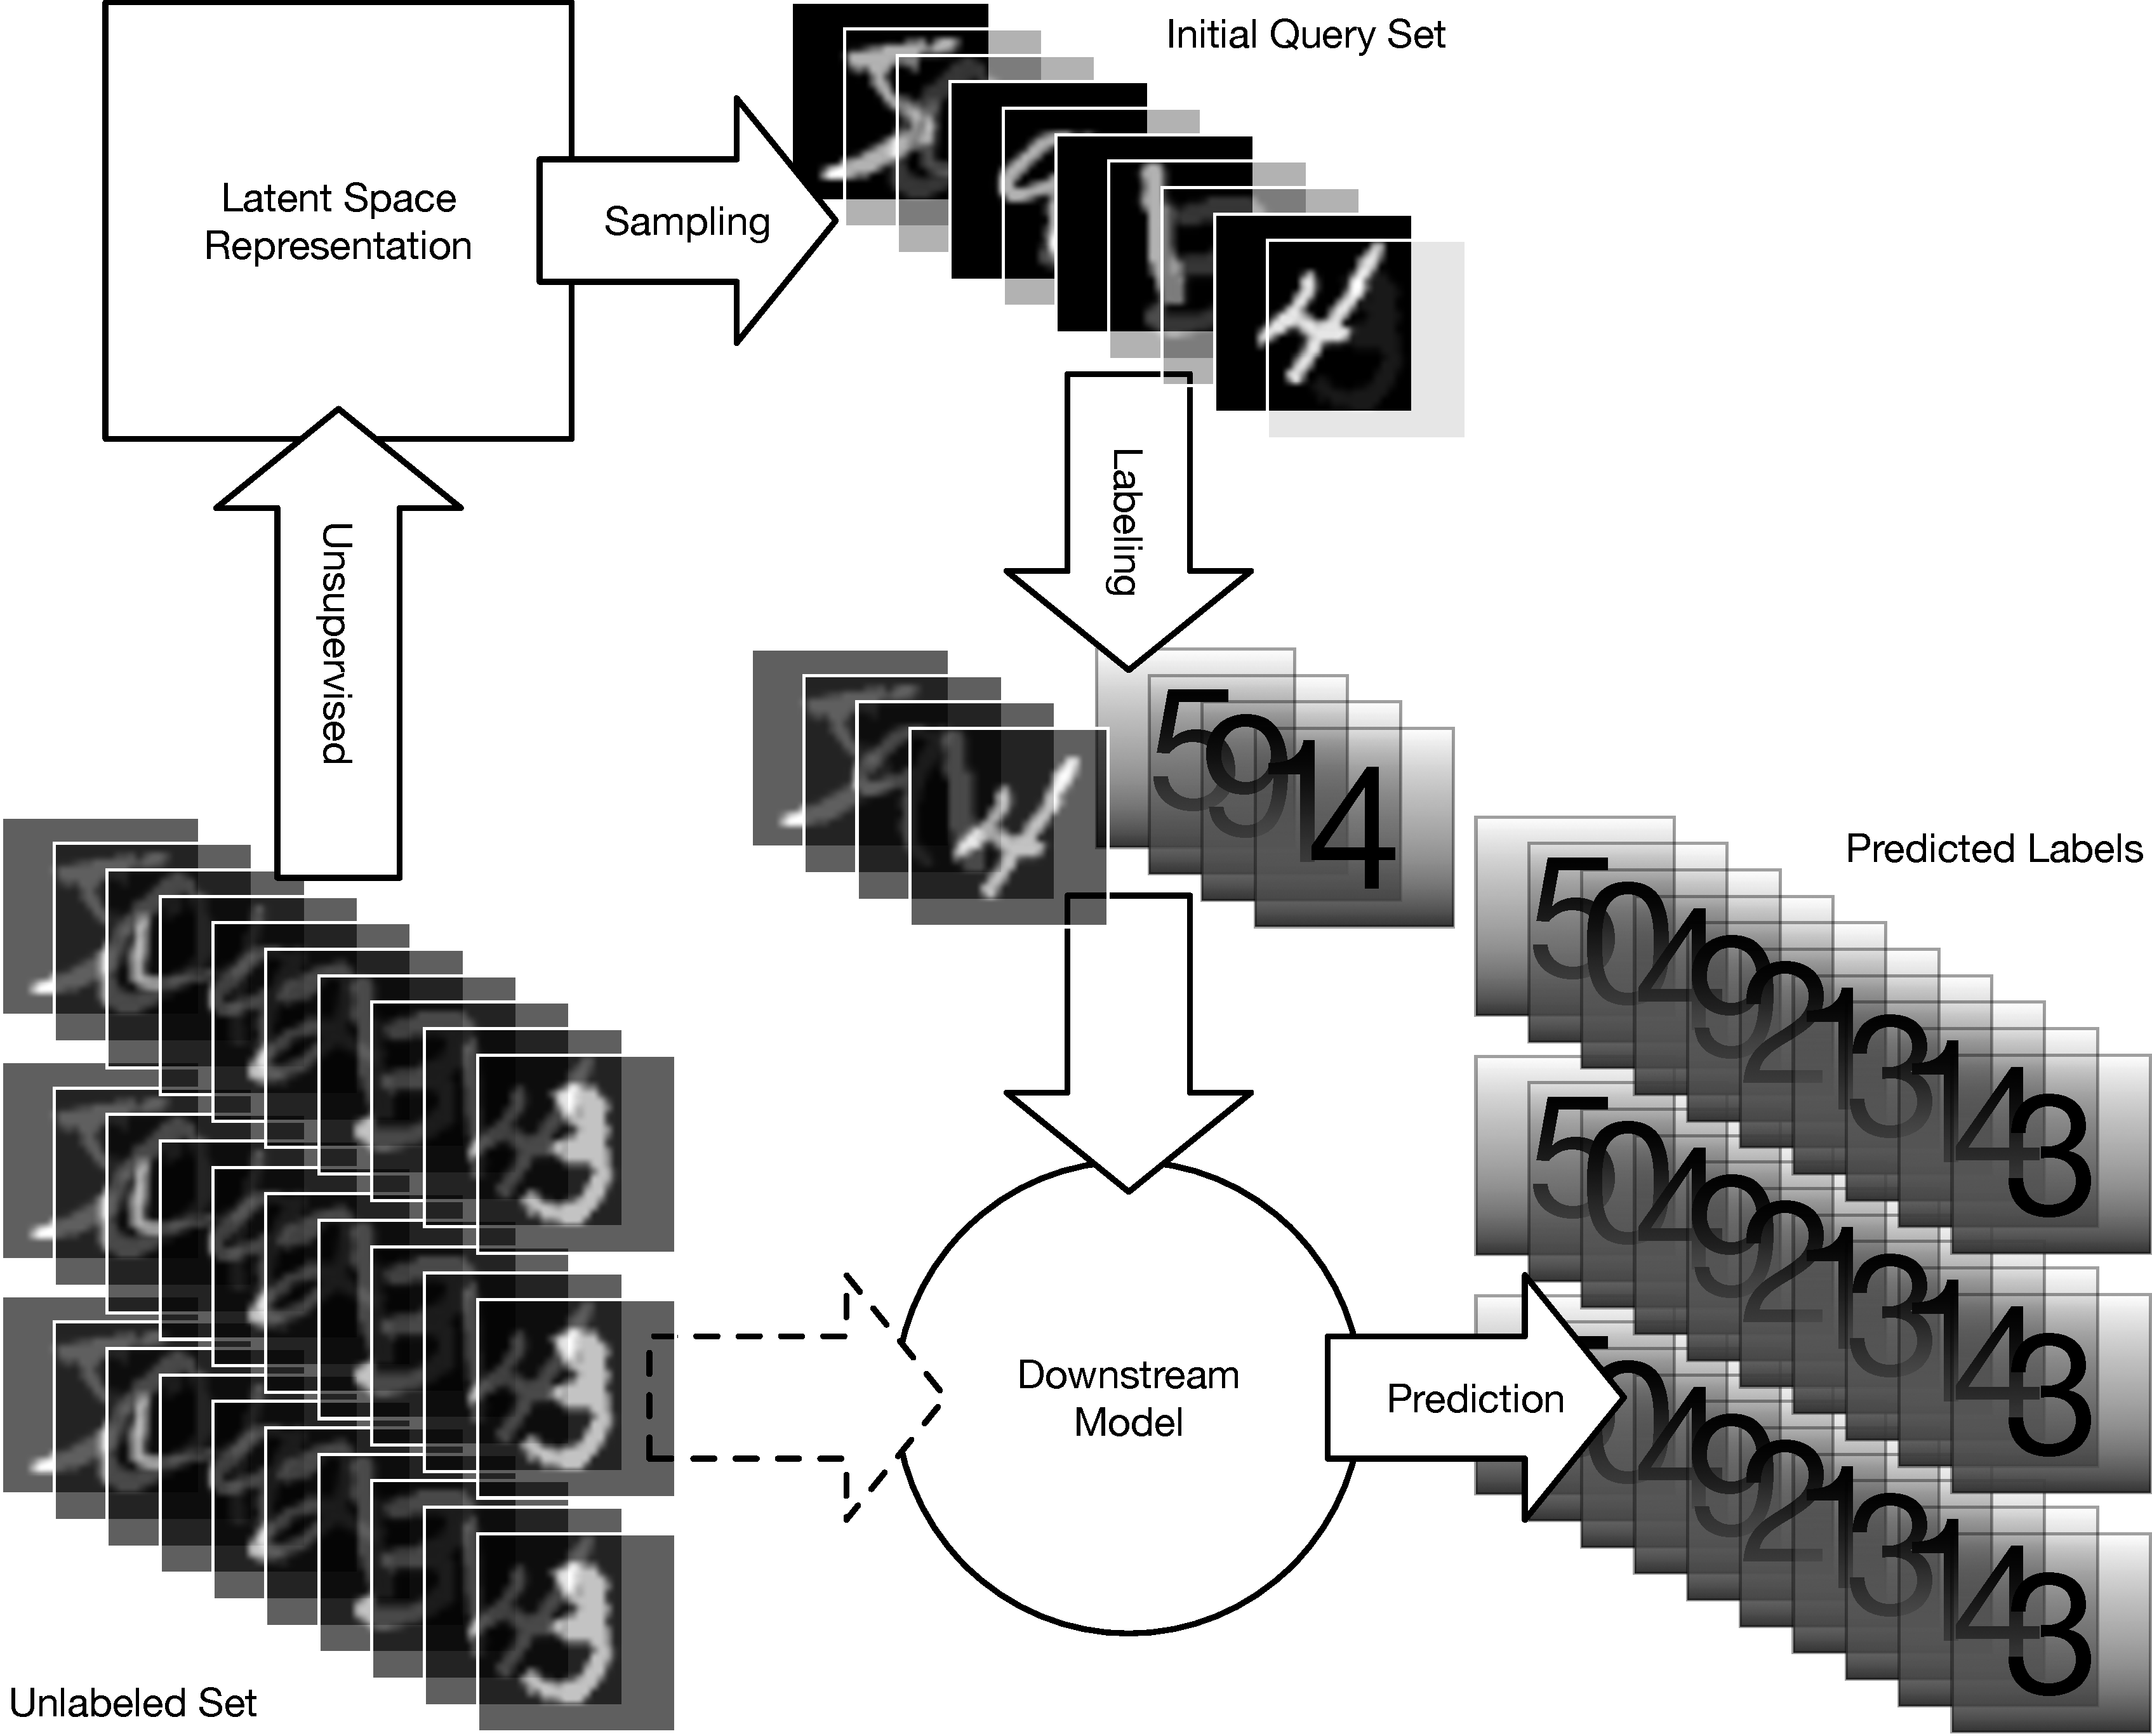
\includegraphics[width=\linewidth]{docs/query_selection}
    \caption{semi-supervised learning.}
    \label{fig:semi-supervised}
  \end{figure}
\end{frame}

\begin{frame}
  \frametitle{Starting from Scratch}
  \begin{columns}
    \column{0.5\textwidth}
    \begin{itemize}
    \item Supervised learning excels where \textbf{labels are available}.
      \pause{}
    \item Many domains require \textbf{starting from scratch} with absolutely no
      labels.
      \pause{}
    \item \emph{e.g.} scientific image analysis.
    \end{itemize}
    \column{0.5\textwidth}
    \begin{figure}
      \centering
      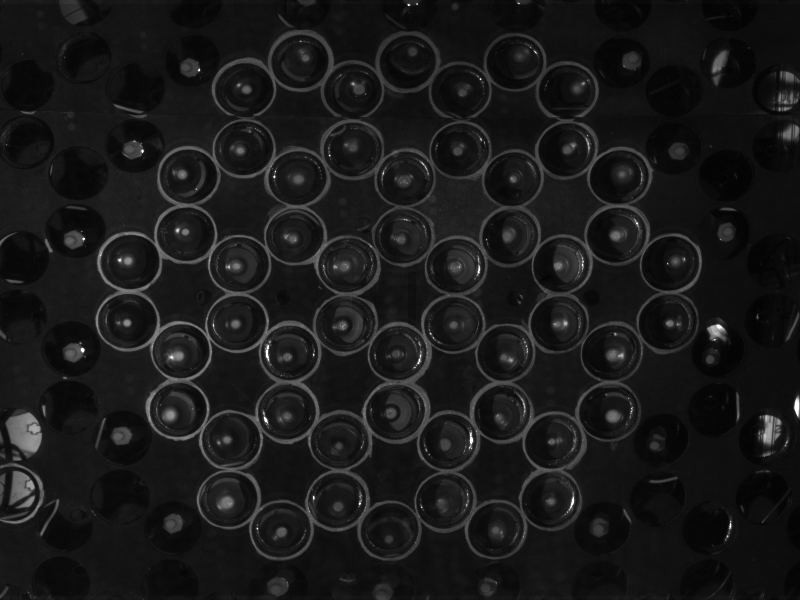
\includegraphics[width=\linewidth]{docs/gyros}
      \caption{gyroscope tracking \cite{nash_topological_2015}.}
      \label{fig:scientific-images}
    \end{figure}
  \end{columns}
\end{frame}


\section{Method}
\label{sec:method}

\begin{frame}
  \frametitle{Method}
  \begin{figure}
    \centering
    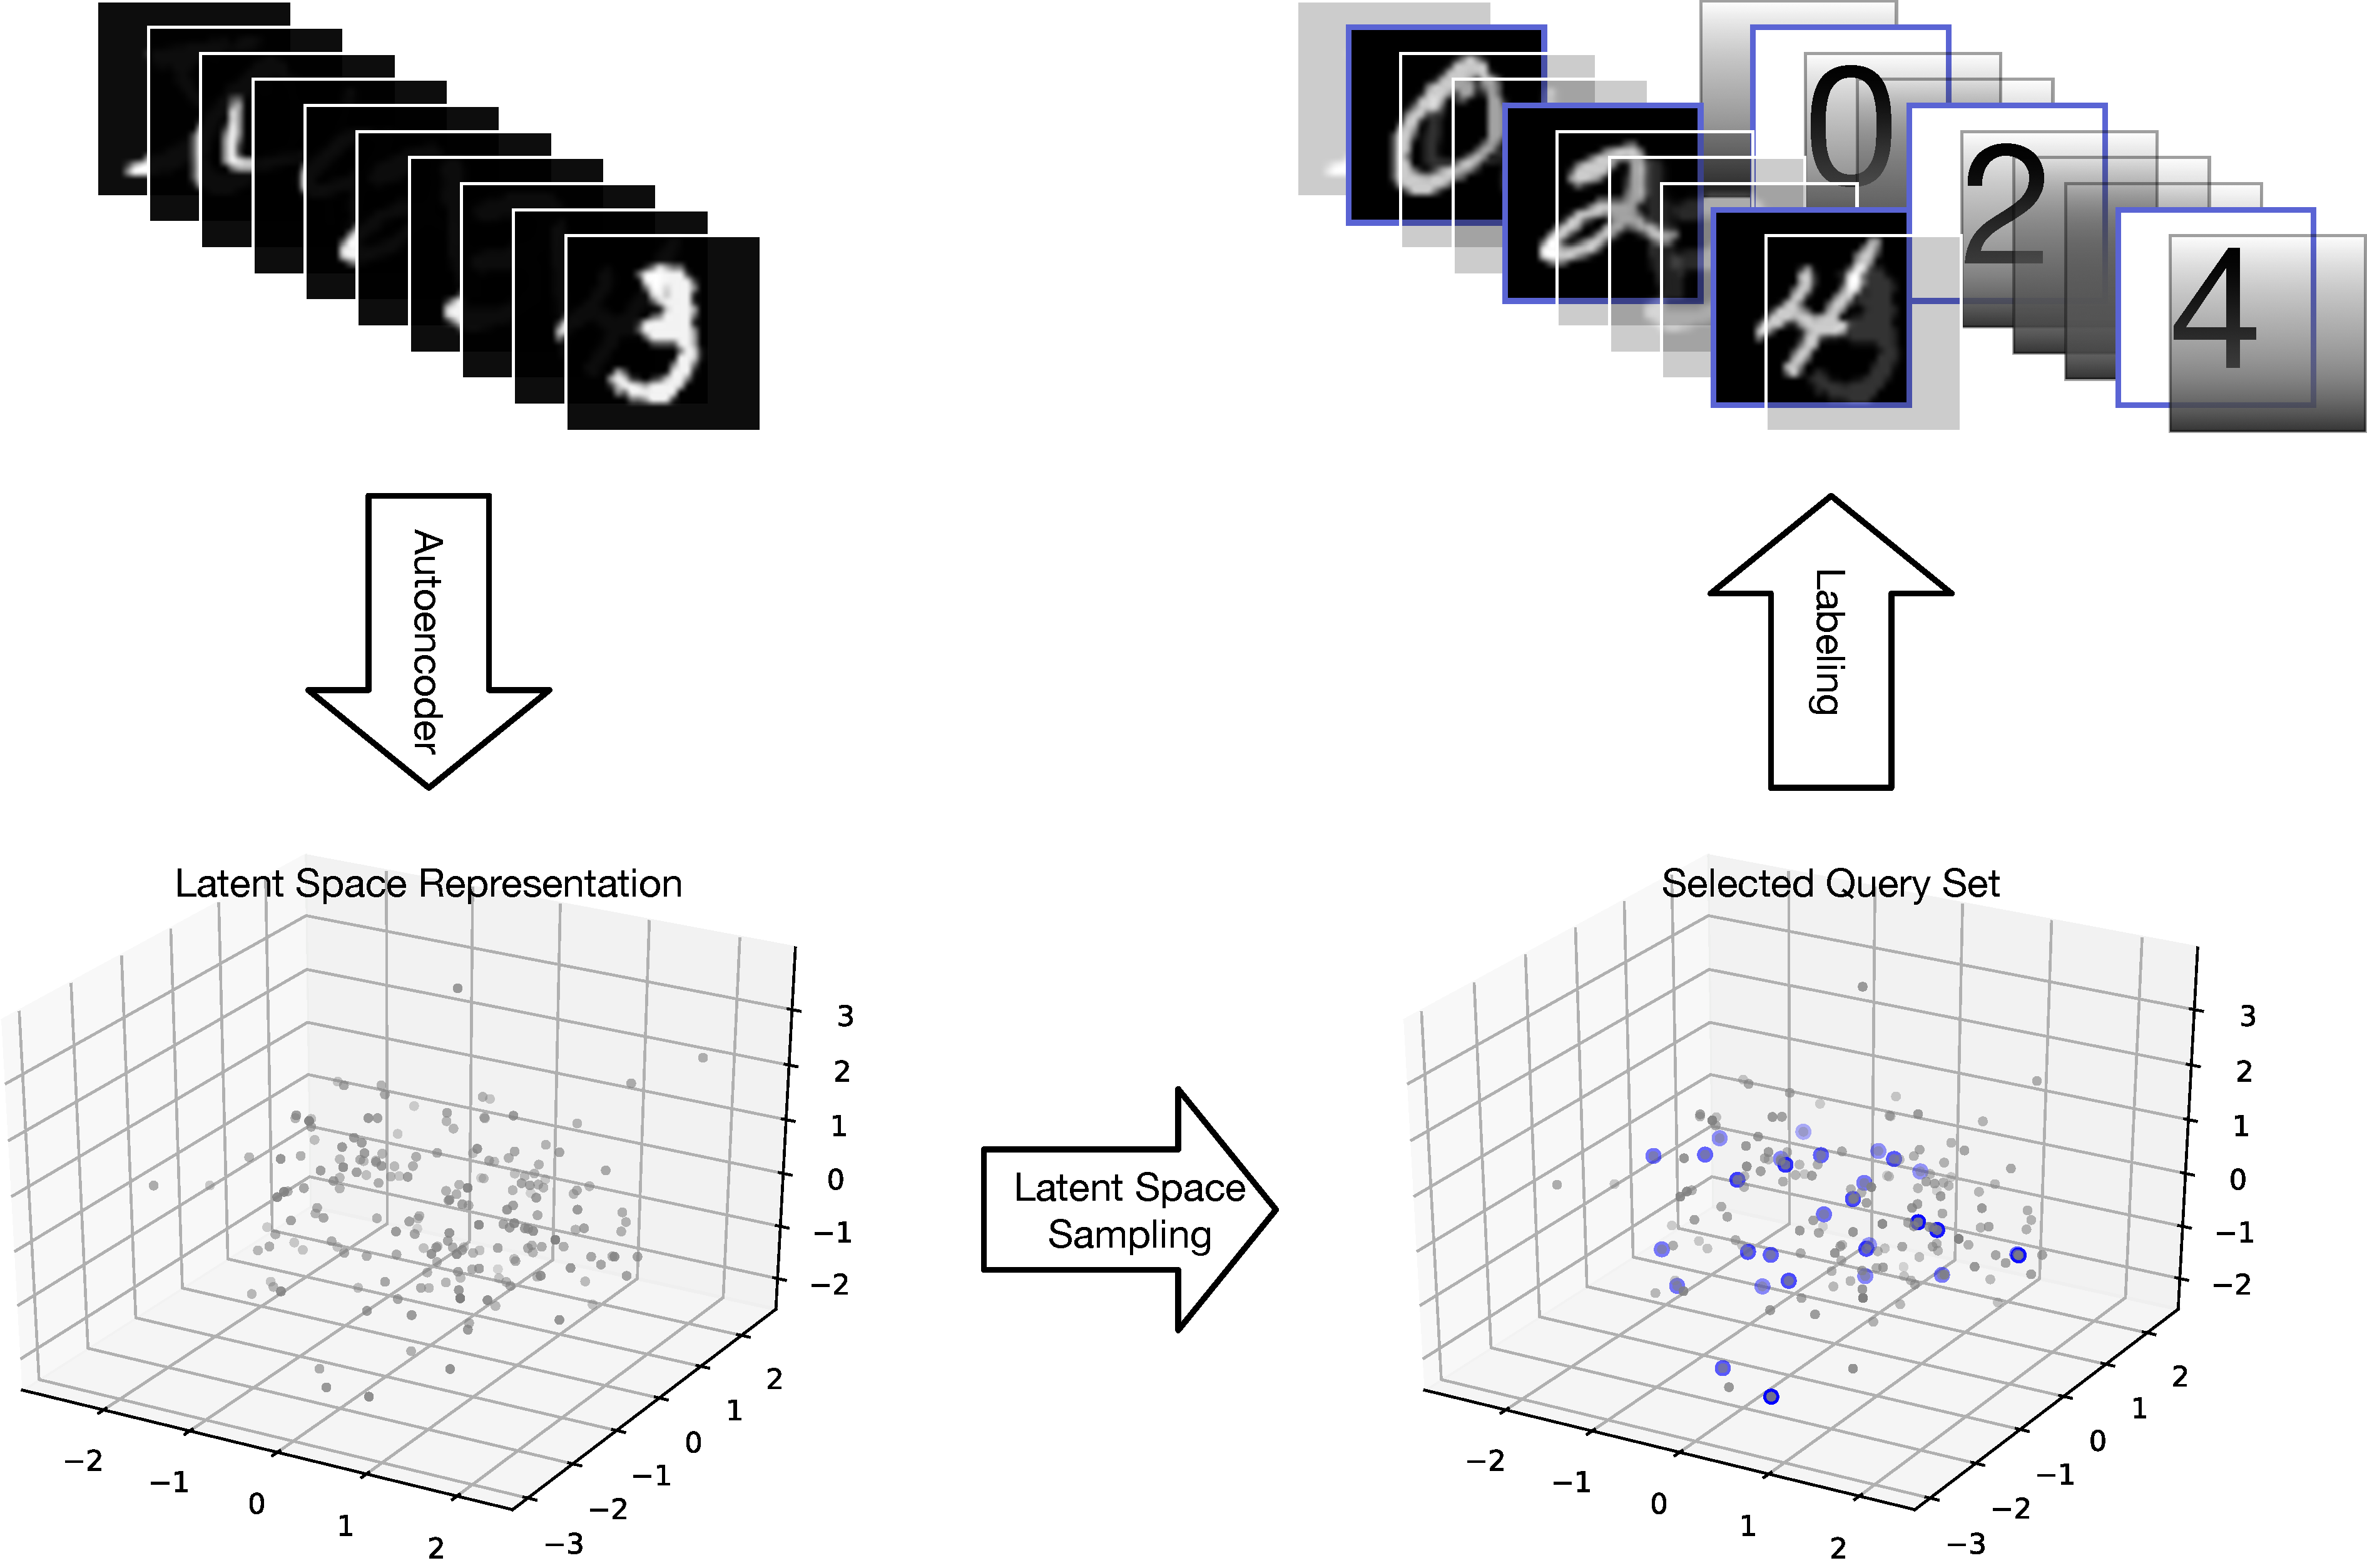
\includegraphics[width=0.8\linewidth]{docs/overview}
    \caption{high-level overview}
    \label{fig:overview}
  \end{figure}
\end{frame}

% \begin{frame}
%   \frametitle{Method}
%   \begin{itemize}
%   \item \textbf{Goal:} explore learned latent space $\mathbb{R}^L$
%     representations for optimal query selection. \pause{}
%   \item \textbf{Constraint:} $L = 2$ \pause{}
%   \item \textbf{Train} multiple auto-encoders:
%     \begin{itemize}
%     \item Convolutional \cite{krizhevsky_imagenet_2012}
%     \item Variational (VAE) \cite{kingma_auto-encoding_2013}
%     \item ``t-SNE style'' \cite{maaten_learning_2009}
%     \item ``Variational t-SNE style''
%     \end{itemize}
%     \pause{}
%   \item \textbf{Explore} multiple sampling strategies:
%     \begin{itemize}
%     \item Distribution based
%     \item Cluster based (hierarchical)
%     \item Performance based
%     \end{itemize}
%   \end{itemize}
% \end{frame}

% \begin{frame}
%   \frametitle{Convolutional Auto-encoder}
%   \begin{itemize}
%   \item $3\times 3$ convolution with 64 kernels (3x)
%   \item $2\times 2$ max-pooling
%   \item $3\times 3$ convolution with 32 kernels (3x)
%   \item $2\times 2$ max-pooling
%   \item $3\times 3$ convolution with 32 kernels (3x)
%   \item $2\times 2$ max-pooling
%   \item 1024-node dense layer (2x)
%   \item $L$-node dense layer, no activation
%   \item 1024-node dense layer (2x)    
%   \item $3\times 3$ convolution with 64 kernels (3x)
%   \item $2\times 2$ transpose convolution
%   \item $3\times 3$ convolution with 32 kernels (3x)
%   \item $2\times 2$ transpose convolution
%   \item $3\times 3$ convolution with 32 kernels (3x)
%   \item $2\times 2$ transpose convolution
%   \end{itemize}
% \end{frame}

% \begin{frame}
%   \frametitle{Architectures}
%   \begin{itemize}
%   \item VAE:
%     \begin{itemize}
%     \item $2L$-node dense layer.
%     \item Normal-distribution sampling layer.
%     \item loss: binary cross-entropy with KL divergence from normal
%       $\kl(Z||\mathcal{N})$.
%     \end{itemize}
%     \pause{}
%   \item ``t-SNE style''
%     \begin{itemize}
%     \item loss: binary cross, entropy with added $\kl(P||Q)$ for batches of 64
%     \end{itemize}
%     \pause{}
%   \item ``Variational t-SNE style'':
%     \begin{itemize}
%     \item $2L$-node dense layer.
%     \item Normal-distribution sampling layer.
%     \item loss: combination of binary cross-entropy, VAE-like
%       $\kl(Z||\mathcal{N})$, and t-SNE style $\kl(P||Q)$.
%     \end{itemize}
%   \end{itemize}
% \end{frame}

% \begin{frame}
%   \frametitle{Sampling}
%   \begin{algorithm}[H]
%     \begin{algorithmic}[1]
%       \Require encoding $Z \in \mathbb{R}^L$, probability distribution
%       $f : \mathbb{R}^L \rightarrow \mathbb{R}$, distance metric
%       $d : \mathbb{R}^{2 \times L} \rightarrow \mathbb{R}$, distance threshold
%       $t \in \mathbb{R}$, $n \in \mathbb{N}$.
      
%       \State $Q \gets \{\}$ %
%       \While {$|Q| < n$} %
%       \State Draw $z \sim f$ %
%       \For {$z_i \in Z$} \Comment the $i$th row of $Z$ %
%       \If {$d(z, z_i) < t$} %
%       \State $Q \gets Q \cup \{i\}$ %
%       \EndIf %
%       \EndFor %
%       \EndWhile %
%       \State %
%       \Return $Q$
%     \end{algorithmic}
%     \caption{Select examples from the encoding $Z$ according to a distribution
%       $f$.}
%     \label{alg:uniform-sampling}
%   \end{algorithm}
% \end{frame}

\section{Results}
\label{sec:results}

\begin{frame}
  \frametitle{Results}
  \begin{columns}
    \column{0.5\textwidth}
    \begin{itemize}
    \item<1-> Reconstructions
    \item<2-> Encodings
    \item<3-> Samplings
    \end{itemize}
    \vspace{1em}
    \includegraphics<2->[width=\linewidth]
    {models/mnist_conv_e300_L2_b64/encodings}
    \column{0.5\textwidth}
    \centering
    \includegraphics<1->[width=\linewidth]
    {models/mnist_conv_e300_L2_b64/reconstruction_1}
    \includegraphics<3->[width=\linewidth]
    {models/mnist_conv_e300_L2_b64/uniform_sampling_1000}
  \end{columns}
\end{frame}


\begin{frame}
  \frametitle{Results}
  \begin{columns}
    \column{0.5\textwidth}
    \begin{itemize}
    \item Reconstructions
    \item Encodings
    \item Samplings
    \end{itemize}
    \vspace{1em}
    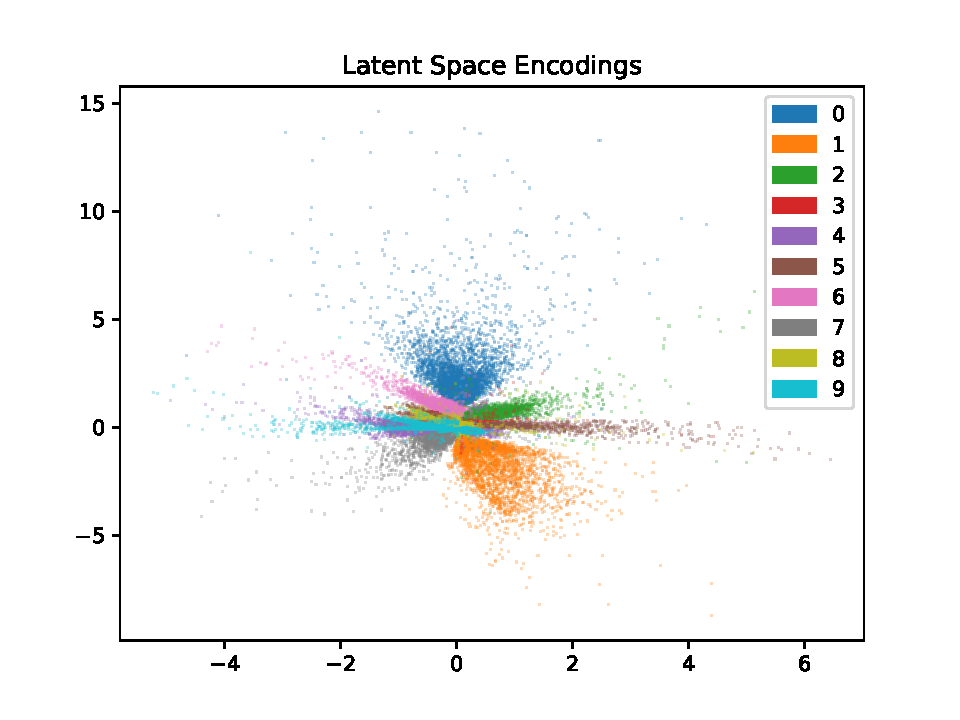
\includegraphics[width=\linewidth]
    {models/mnist_conv_e300_L2_b64/encodings}
    \column{0.5\textwidth}
    \centering
    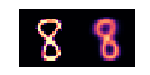
\includegraphics[width=\linewidth]
    {models/mnist_conv_e300_L2_b64/reconstruction_1} \\
    \vspace{2em}
    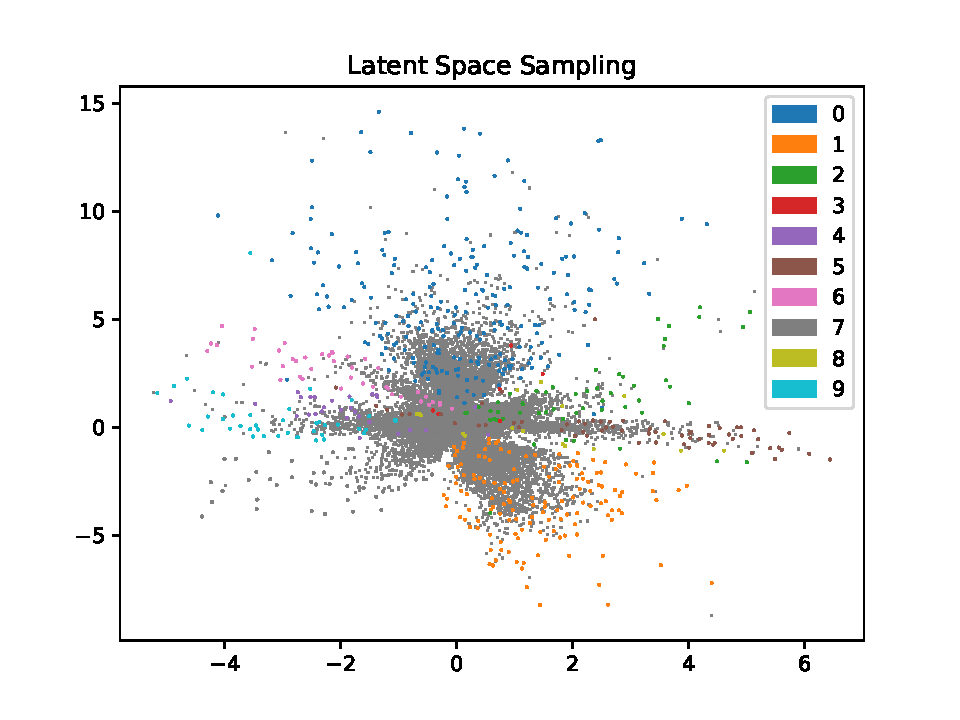
\includegraphics[width=\linewidth]
    {models/mnist_conv_e300_L2_b64/uniform_sampling_1000}
  \end{columns}
\end{frame}


\subsection{Convolutional AE}

\begin{frame}
  \frametitle{Convolutional Auto-encoder}
  \begin{columns}
    \column{0.5\textwidth}
    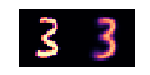
\includegraphics[width=\linewidth]
    {models/mnist_conv_e300_L2_b64/reconstruction_0} \\
    \vspace{2em}
    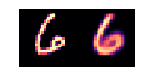
\includegraphics[width=\linewidth]
    {models/mnist_conv_e300_L2_b64/reconstruction_2}
    \column{0.5\textwidth}
    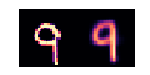
\includegraphics[width=\linewidth]
    {models/mnist_conv_e300_L2_b64/reconstruction_3} \\
    \vspace{2em}
    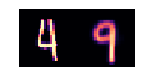
\includegraphics[width=\linewidth]
    {models/mnist_conv_e300_L2_b64/reconstruction_5}
  \end{columns}
\end{frame}

\begin{frame}
  \frametitle{Convolutional Auto-encoder}
  \begin{figure}
    \centering
    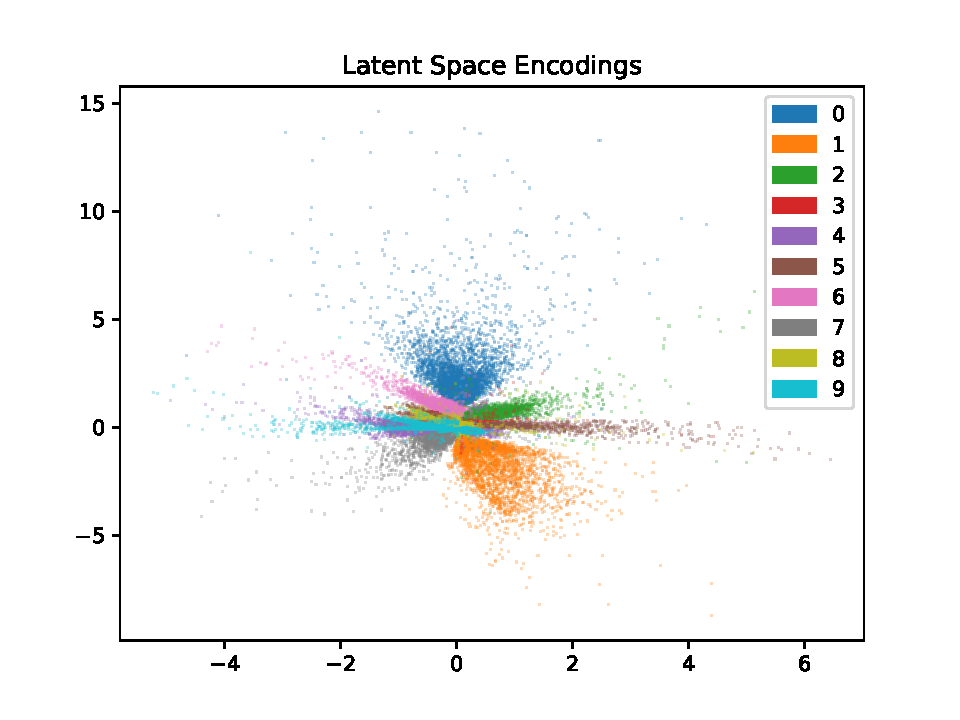
\includegraphics[width=\linewidth]
    {models/mnist_conv_e300_L2_b64/encodings}
    \caption{}
    \label{fig:conv-encodings}
  \end{figure}
\end{frame}

\begin{frame}
  \frametitle{Uniform Spatial Sampling}
  \begin{figure}
    \centering
    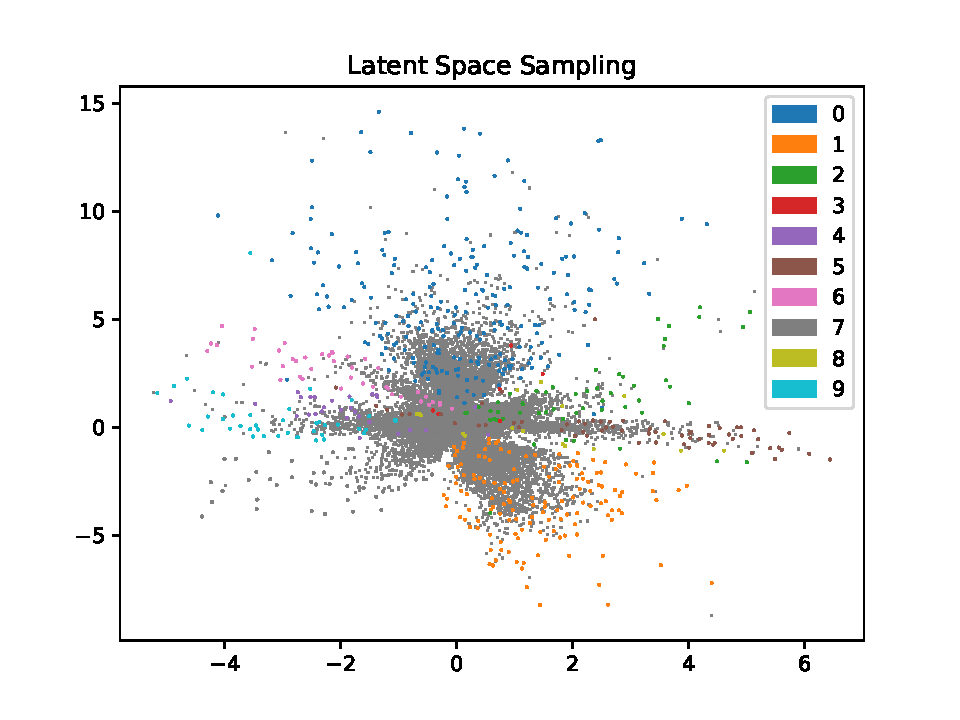
\includegraphics[width=\linewidth]
    {models/mnist_conv_e300_L2_b64/uniform_sampling_1000}
    \caption{}
    \label{fig:conv-uniform}
  \end{figure}
\end{frame}

\begin{frame}
  \frametitle{Uniform Spatial Sampling}
  \begin{figure}
    \centering
    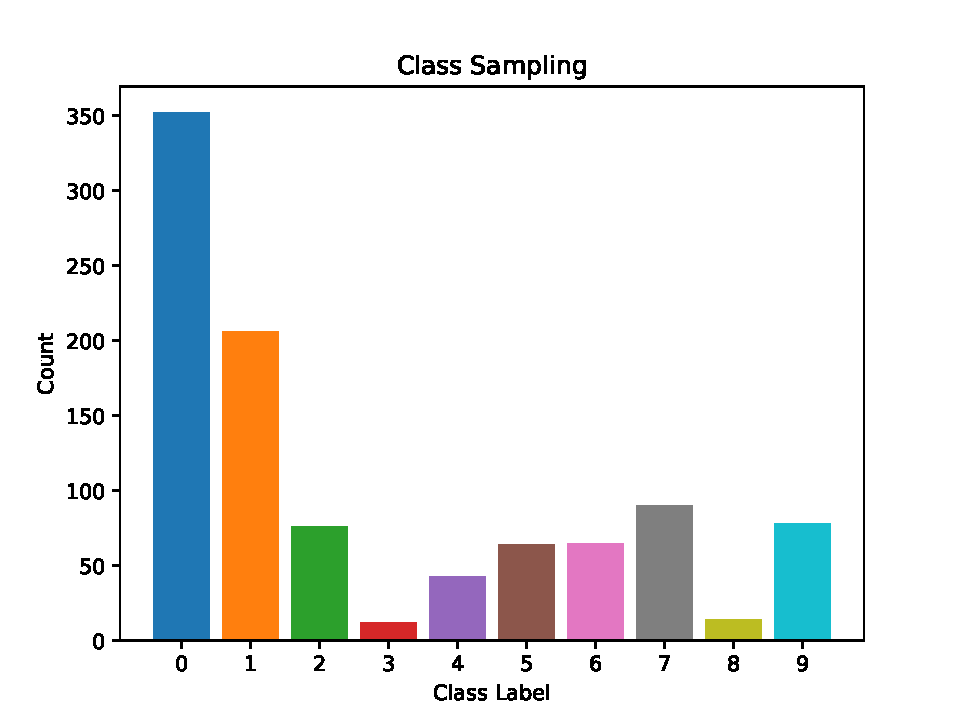
\includegraphics[width=\linewidth]
    {models/mnist_conv_e300_L2_b64/uniform_sampling_distribution_1000}
    \caption{}
    \label{fig:conv-uniform}
  \end{figure}
\end{frame}

% \begin{frame}
%   \frametitle{Normal Spatial Sampling}
%   \begin{figure}
%     \centering
%     \includegraphics[width=\linewidth]
%     {models/mnist_conv_e300_L2_b64/normal_sampling_1000}
%     \caption{}
%     \label{}
%   \end{figure}
% \end{frame}

% \begin{frame}
%   \frametitle{Normal Spatial Sampling}
%   \begin{figure}
%     \centering
%     \includegraphics[width=\linewidth]
%     {models/mnist_conv_e300_L2_b64/normal_sampling_distribution_1000}
%     \caption{}
%     \label{}
%   \end{figure}
% \end{frame}

% \begin{frame}
%   \frametitle{Clustering}
%   \begin{figure}
%     \centering
%     \includegraphics[width=\linewidth]
%     {models/mnist_conv_e300_L2_b64/uniform-cluster_clustered_encodings}
%     \caption{}
%     \label{}
%   \end{figure}
% \end{frame}

% \begin{frame}
%   \frametitle{Cluster Sampling}
%   \begin{figure}
%     \centering
%     \includegraphics[width=\linewidth]
%     {models/mnist_conv_e300_L2_b64/uniform-cluster_sampling_1000}
%     \caption{}
%     \label{}
%   \end{figure}
% \end{frame}

% \begin{frame}
%   \frametitle{Cluster Sampling}
%   \begin{figure}
%     \centering
%     \includegraphics[width=\linewidth]
%     {models/mnist_conv_e300_L2_b64/uniform-cluster_sampling_distribution_1000}
%     \caption{}
%     \label{}
%   \end{figure}
% \end{frame}

% \begin{frame}
%   \frametitle{Normal Sampling inside Clusters}
%   \begin{figure}
%     \centering
%     \includegraphics[width=\linewidth]
%     {models/mnist_conv_e300_L2_b64/multi-normal-cluster_sampling_1000}
%     \caption{}
%     \label{}
%   \end{figure}
% \end{frame}

% \begin{frame}
%   \frametitle{Normal Sampling inside Clusters}
%   \begin{figure}
%     \centering
%     \includegraphics[width=\linewidth]
%     {models/mnist_conv_e300_L2_b64/multi-normal-cluster_sampling_distribution_1000}
%     \caption{}
%     \label{}
%   \end{figure}
% \end{frame}

\subsection{Variational AE}

% \begin{frame}
%   \frametitle{Variational Auto-encoder}
%   \begin{columns}
%     \column{0.5\textwidth}
%     \includegraphics[width=\linewidth]
%     {models/mnist_vae_e300_L2_b64/reconstruction_0} \\
%     \vspace{2em}
%     \includegraphics[width=\linewidth]
%     {models/mnist_vae_e300_L2_b64/reconstruction_2}
%     \column{0.5\textwidth}
%     \includegraphics[width=\linewidth]
%     {models/mnist_vae_e300_L2_b64/reconstruction_3} \\
%     \vspace{2em}
%     \includegraphics[width=\linewidth]
%     {models/mnist_vae_e300_L2_b64/reconstruction_5}
%   \end{columns}
% \end{frame}

\begin{frame}
  \frametitle{Variational Auto-encoder}
  \begin{figure}
    \centering
    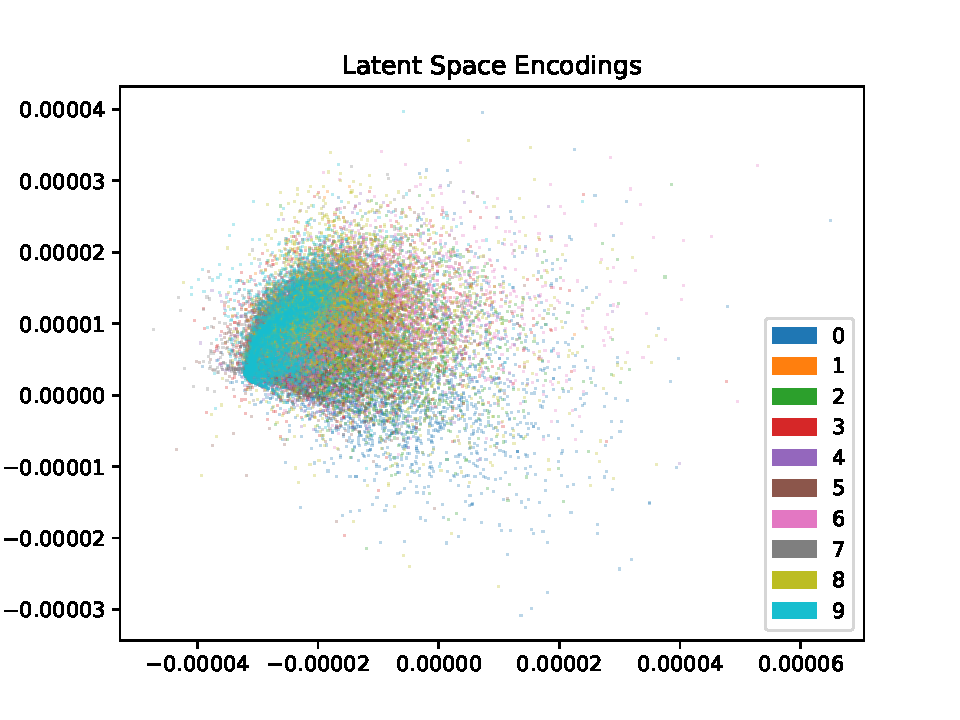
\includegraphics[width=\linewidth]
    {models/mnist_vae_e300_L2_b64/encodings}
    \caption{}
    \label{}
  \end{figure}
\end{frame}

\begin{frame}
  \frametitle{Normal Spatial Sampling}
  \begin{figure}
    \centering
    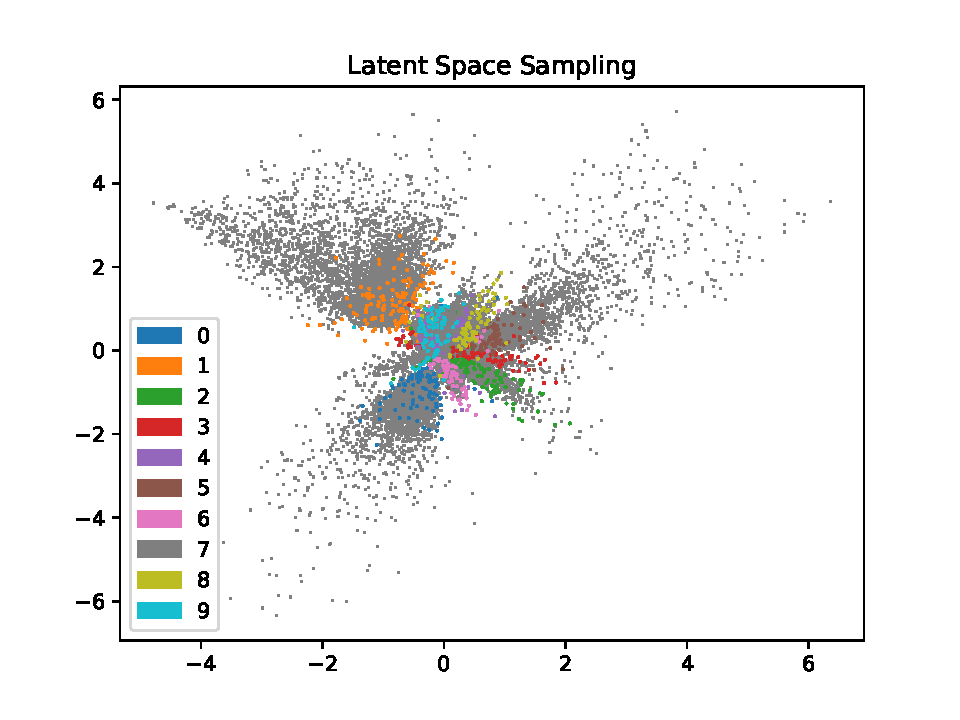
\includegraphics[width=\linewidth]
    {models/mnist_vae_e300_L2_b64/multi-normal_sampling_1000}
    \caption{}
    \label{}
  \end{figure}
\end{frame}

\begin{frame}
  \frametitle{Normal Spatial Sampling}
  \begin{figure}
    \centering
    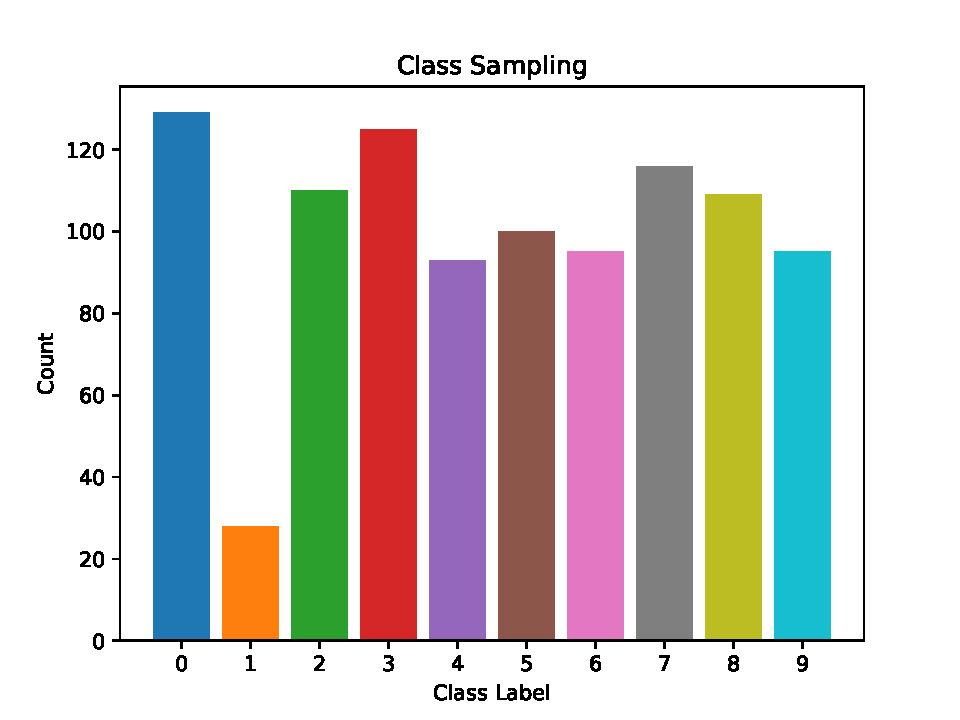
\includegraphics[width=\linewidth]
    {models/mnist_vae_e300_L2_b64/multi-normal_sampling_distribution_1000}
    \caption{}
    \label{}
  \end{figure}
\end{frame}

\subsection{t-SNE Style AE}

% \begin{frame}
%   \frametitle{t-SNE Style Auto-encoder}
%   \begin{columns}
%     \column{0.5\textwidth}
%     \includegraphics[width=\linewidth]
%     {models/mnist_student_e300_L2_b64/reconstruction_0} \\
%     \vspace{2em}
%     \includegraphics[width=\linewidth]
%     {models/mnist_student_e300_L2_b64/reconstruction_2}
%     \column{0.5\textwidth}
%     \includegraphics[width=\linewidth]
%     {models/mnist_student_e300_L2_b64/reconstruction_3} \\
%     \vspace{2em}
%     \includegraphics[width=\linewidth]
%     {models/mnist_student_e300_L2_b64/reconstruction_5}
%   \end{columns}
% \end{frame}

\begin{frame}
  \frametitle{t-SNE Style Auto-encoder}
  \begin{figure}
    \centering
    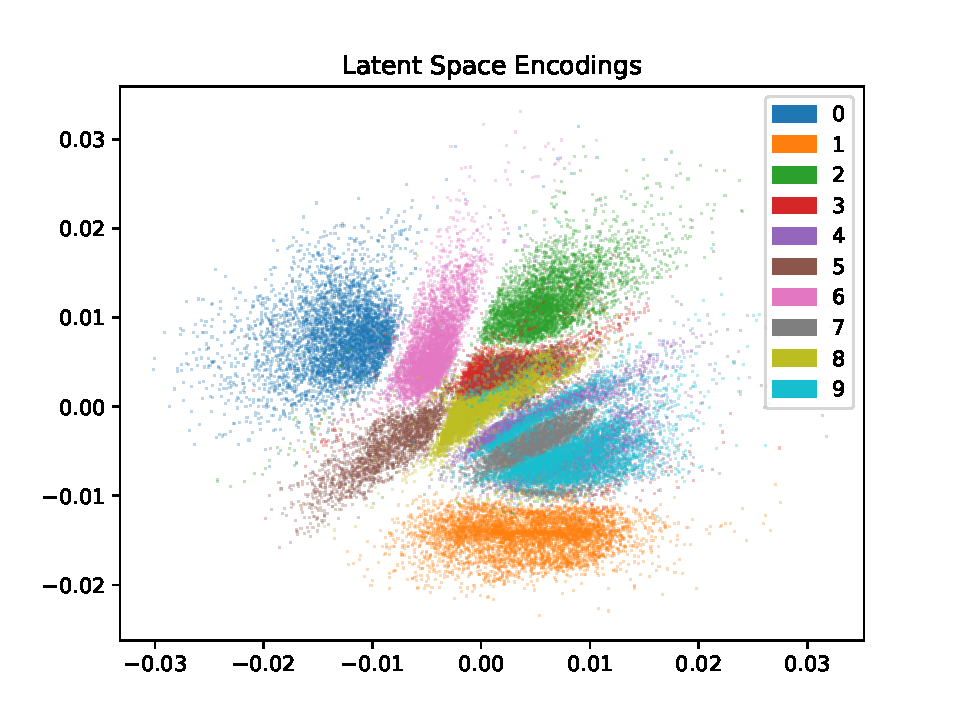
\includegraphics[width=\linewidth]
    {models/mnist_student_e300_L2_b64/encodings}
    \caption{}
    \label{}
  \end{figure}
\end{frame}

\begin{frame}
  \frametitle{Clustering}
  \begin{figure}
    \centering
    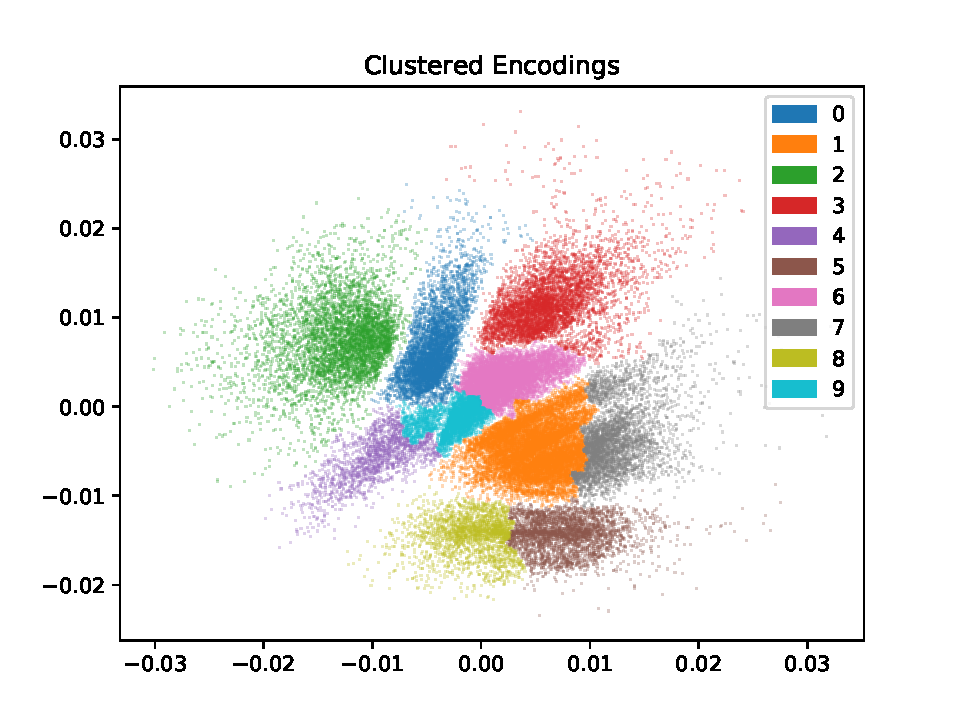
\includegraphics[width=\linewidth]
    {models/mnist_student_e300_L2_b64/multi-normal-cluster_clustered_encodings}
    \caption{}
    \label{}
  \end{figure}
\end{frame}

\begin{frame}
  \frametitle{Normal Sampling inside Clusters}
  \begin{figure}
    \centering
    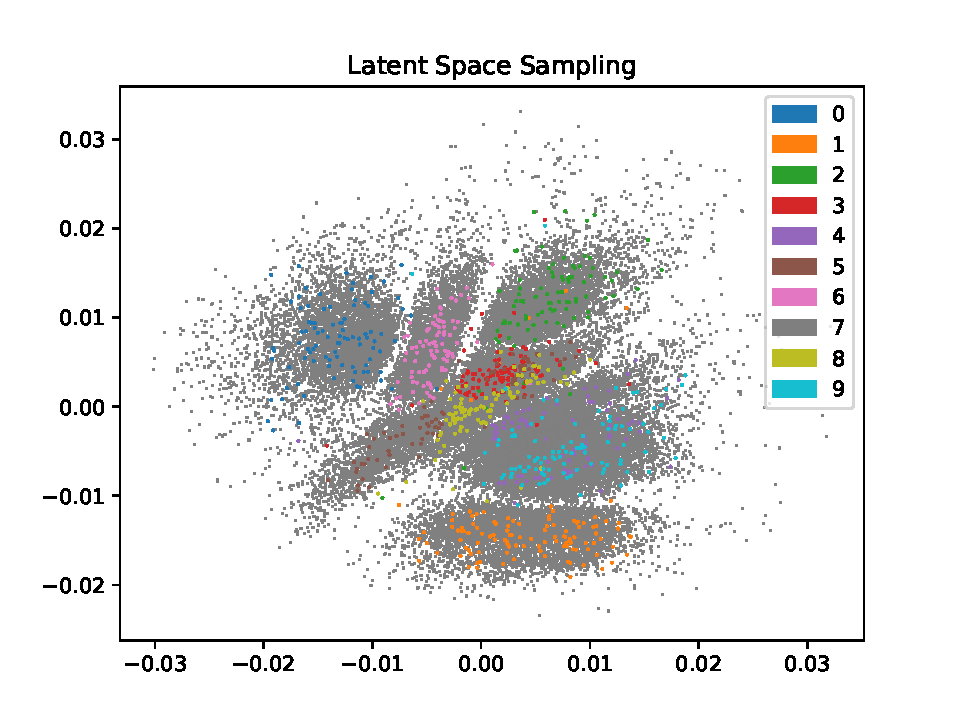
\includegraphics[width=\linewidth]
    {models/mnist_student_e300_L2_b64/multi-normal-cluster_sampling_1000}
    \caption{}
    \label{}
  \end{figure}
\end{frame}

\begin{frame}
  \frametitle{Clustered Normal Spatial Sampling}
  \begin{figure}
    \centering
    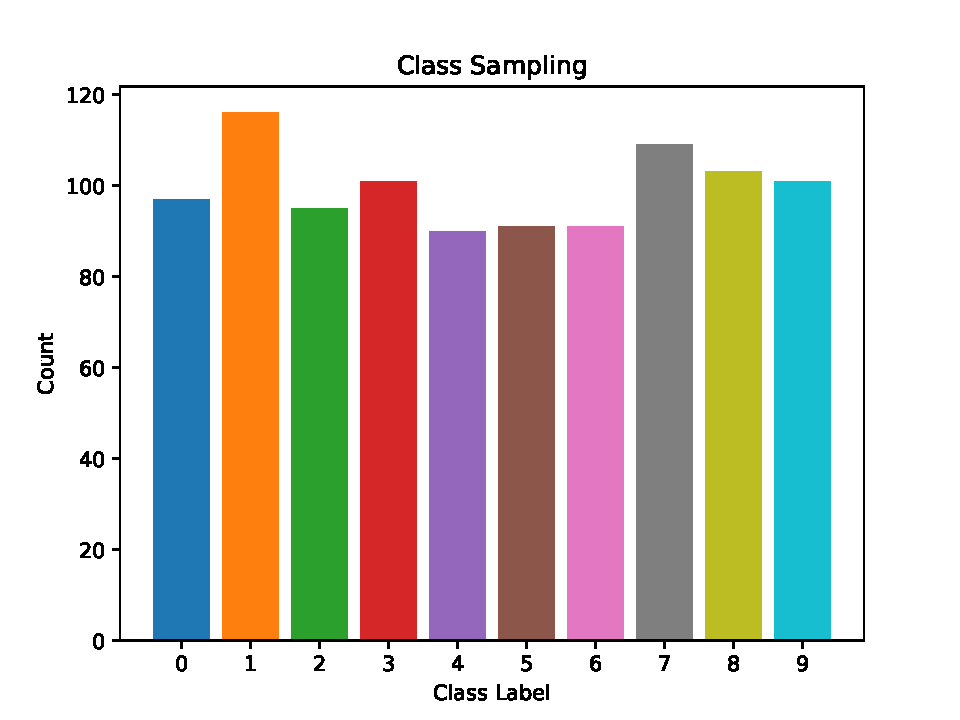
\includegraphics[width=\linewidth]
    {models/mnist_student_e300_L2_b64/multi-normal-cluster_sampling_distribution_1000}
    \caption{}
    \label{}
  \end{figure}
\end{frame}

% \subsection{Variational t-SNE Style AE}

% \begin{frame}
%   \frametitle{Variational t-SNE Style Auto-encoder}
%   \begin{columns}
%     \column{0.5\textwidth}
%     \includegraphics[width=\linewidth]
%     {models/mnist_vaestudent_e300_L2_b64/reconstruction_0} \\
%     \vspace{2em}
%     \includegraphics[width=\linewidth]
%     {models/mnist_vaestudent_e300_L2_b64/reconstruction_2}
%     \column{0.5\textwidth}
%     \includegraphics[width=\linewidth]
%     {models/mnist_vaestudent_e300_L2_b64/reconstruction_3} \\
%     \vspace{2em}
%     \includegraphics[width=\linewidth]
%     {models/mnist_vaestudent_e300_L2_b64/reconstruction_5}
%   \end{columns}
% \end{frame}

% \begin{frame}
%   \frametitle{Variational t-SNE Style Auto-encoder}
%   \begin{figure}
%     \centering
%     \includegraphics[width=\linewidth]
%     {models/mnist_vaestudent_e300_L2_b64/encodings}
%     \caption{}
%     \label{}
%   \end{figure}
% \end{frame}


% \begin{frame}
%   \frametitle{Normal Sampling inside Clusters}
%   \begin{figure}
%     \centering
%     \includegraphics[width=\linewidth]
%     {models/mnist_vaestudent_e300_L2_b64/multi-normal-cluster_sampling_1000}
%     \caption{}
%     \label{}
%   \end{figure}
% \end{frame}

% \begin{frame}
%   \frametitle{Clustered Normal Spatial Sampling}
%   \begin{figure}
%     \centering
%     \includegraphics[width=\linewidth]
%     {models/mnist_vaestudent_e300_L2_b64/multi-normal-cluster_sampling_distribution_1000}
%     \caption{}
%     \label{}
%   \end{figure}
% \end{frame}


% \subsection{Reconstruction Error Sampling}

% \begin{frame}
%   \frametitle{Reconstruction Error Sampling}
%   \begin{figure}
%     \centering
%     \includegraphics[width=\linewidth]
%     {models/mnist_student_e300_L2_b64/error_sampling_1000}
%     \caption{}
%     \label{}
%   \end{figure}  
% \end{frame}

% \begin{frame}
%   \frametitle{Reconstruction Error Sampling}
%   \begin{figure}
%     \centering
%     \includegraphics[width=\linewidth]
%     {models/mnist_student_e300_L2_b64/error_sampling_distribution_1000}
%     \caption{}
%     \label{}
%   \end{figure}  
% \end{frame}

\section{Discussion}
\begin{frame}
  \frametitle{Discussion}
  \begin{itemize}
  \item Normal sampling inside clusters yields \textbf{balanced samples}. \pause{}
  \item Are auto-encoders the \textbf{best choice} for latent-space
    representation?\pause{}
  \item Distribution of \textbf{difficult examples} in latent space.
  \end{itemize}
  \pause
  \begin{figure}
    \centering
    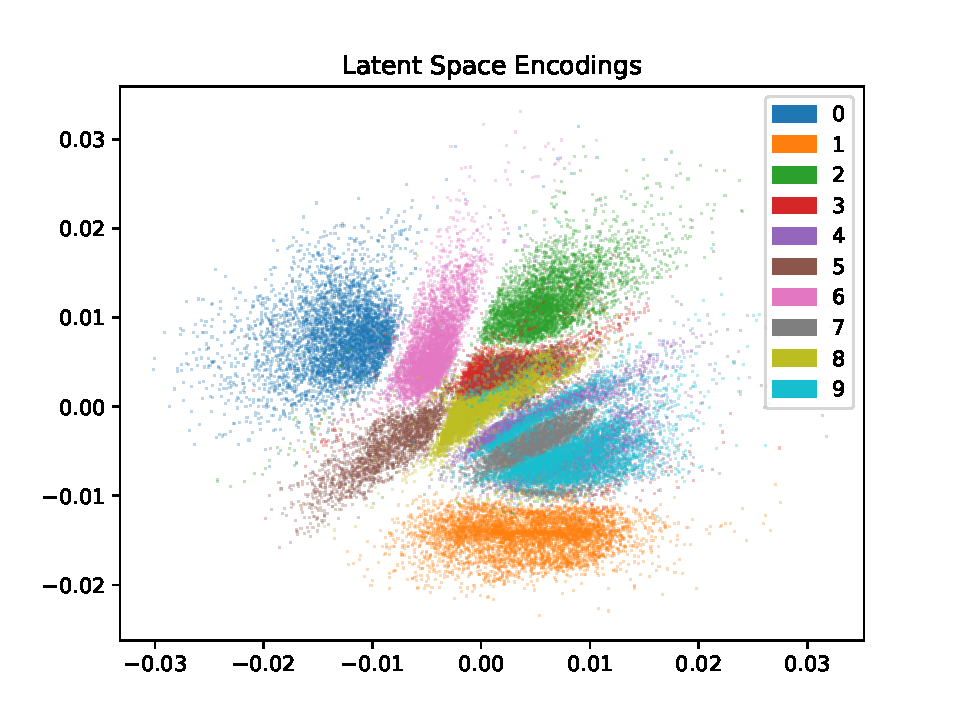
\includegraphics[width=0.49\linewidth]
    {models/mnist_student_e300_L2_b64/encodings}
    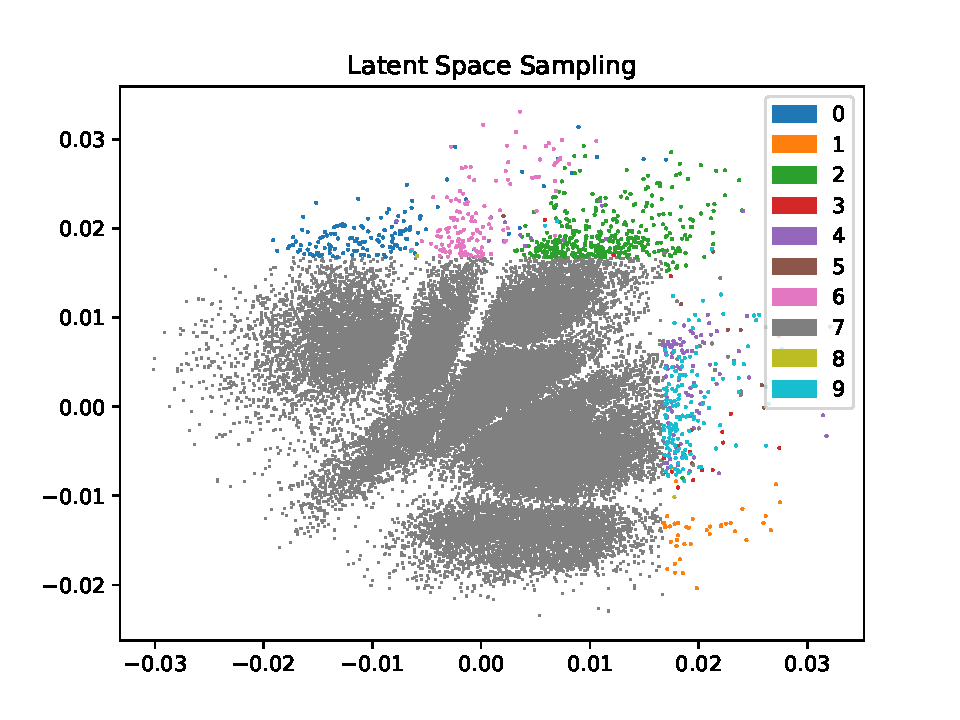
\includegraphics[width=0.49\linewidth]
    {models/mnist_student_e300_L2_b64/classifier-loss_sampling_1000}
    \caption{Visualizing points which are difficult to learn.}
    \label{}
  \end{figure}
\end{frame}

\section{Future Work}
\begin{frame}
  \frametitle{Future Work}
  \begin{itemize}
  \item<1-> Transfer learning \textbf{without overfitting}.
  \item<2-> Evaluate performance of classifiers \textbf{trained on query
      selections}.
  \item<3-> Explore higher dimensions.
  \item<4-> Labeling \textbf{artificial examples} produced by an auto-encoder.
  \end{itemize}
\end{frame}

\section{References}
\label{sec:references}

\begin{frame}[t, allowframebreaks]
  \frametitle{References}
  \tiny
  \bibliographystyle{IEEEtran}
  \bibliography{presentation}
\end{frame}

\end{document}

Full classifier output:
\begin{verbatim}
Epoch 1/10
781/782 [============================>.] - ETA: 0s - loss: 0.5675 - acc: 0.8668
782/782 [==============================] - 11s 14ms/step - loss: 0.5670 - acc: 0.8669 - val_loss: 0.2813 - val_acc: 0.9219
Epoch 2/10
781/782 [============================>.] - ETA: 0s - loss: 0.2607 - acc: 0.9270
782/782 [==============================] - 7s 9ms/step - loss: 0.2607 - acc: 0.9269 - val_loss: 0.2217 - val_acc: 0.9395
Epoch 3/10
780/782 [============================>.] - ETA: 0s - loss: 0.2108 - acc: 0.9406
782/782 [==============================] - 7s 9ms/step - loss: 0.2107 - acc: 0.9407 - val_loss: 0.1884 - val_acc: 0.9454
Epoch 4/10
780/782 [============================>.] - ETA: 0s - loss: 0.1794 - acc: 0.9490
782/782 [==============================] - 7s 9ms/step - loss: 0.1792 - acc: 0.9490 - val_loss: 0.1678 - val_acc: 0.9512
Epoch 5/10
779/782 [============================>.] - ETA: 0s - loss: 0.1563 - acc: 0.9558
782/782 [==============================] - 7s 9ms/step - loss: 0.1561 - acc: 0.9558 - val_loss: 0.1481 - val_acc: 0.9578
Epoch 6/10
778/782 [============================>.] - ETA: 0s - loss: 0.1391 - acc: 0.9607
782/782 [==============================] - 7s 9ms/step - loss: 0.1393 - acc: 0.9606 - val_loss: 0.1402 - val_acc: 0.9601
Epoch 7/10
777/782 [============================>.] - ETA: 0s - loss: 0.1243 - acc: 0.9647
782/782 [==============================] - 7s 9ms/step - loss: 0.1240 - acc: 0.9648 - val_loss: 0.1263 - val_acc: 0.9638
Epoch 8/10
777/782 [============================>.] - ETA: 0s - loss: 0.1131 - acc: 0.9685
782/782 [==============================] - 7s 9ms/step - loss: 0.1129 - acc: 0.9686 - val_loss: 0.1178 - val_acc: 0.9655
Epoch 9/10
776/782 [============================>.] - ETA: 0s - loss: 0.1026 - acc: 0.9716
782/782 [==============================] - 8s 11ms/step - loss: 0.1024 - acc: 0.9717 - val_loss: 0.1109 - val_acc: 0.9670
Epoch 10/10
775/782 [============================>.] - ETA: 0s - loss: 0.0945 - acc: 0.9742
782/782 [==============================] - 7s 9ms/step - loss: 0.0942 - acc: 0.9743 - val_loss: 0.1056 - val_acc: 0.9686
157/157 [==============================] - 3s 20ms/step
INFO:latens:test accuracy: 97.1%
\end{verbatim}

%%% Local Variables:
%%% mode: latex
%%% TeX-master: t
%%% End:
